 \section{Actividad – Crear relaciones} 
Para crear los informes en Power BI Desktop, primero debe conectarse a los datos y después darles forma. Después podrá guardar los informes en el formato de archivos de Power BI Desktop, que es la extensión .pbix. Y también va a poder compartirlos. Puede hacerlo como cualquier otro archivo, pero sin duda como va a aprovechar todo su potencial será si lo comparte desde el servicio de Power Bi.
\begin{itemize}
	\item Conectarse a datos: normalmente son varios orígenes de datos.
	\item Dar forma a dichos datos: mediante las consultas que crean modelos de datos precisos.
	\item Crear informes: usando modelos que otros pueden aprovechar, compartir y usar como punto de partida.\\
\end{itemize} 

\begin{itemize}
	\item Resultado del Modelo en Power BI 
	\begin{center}
	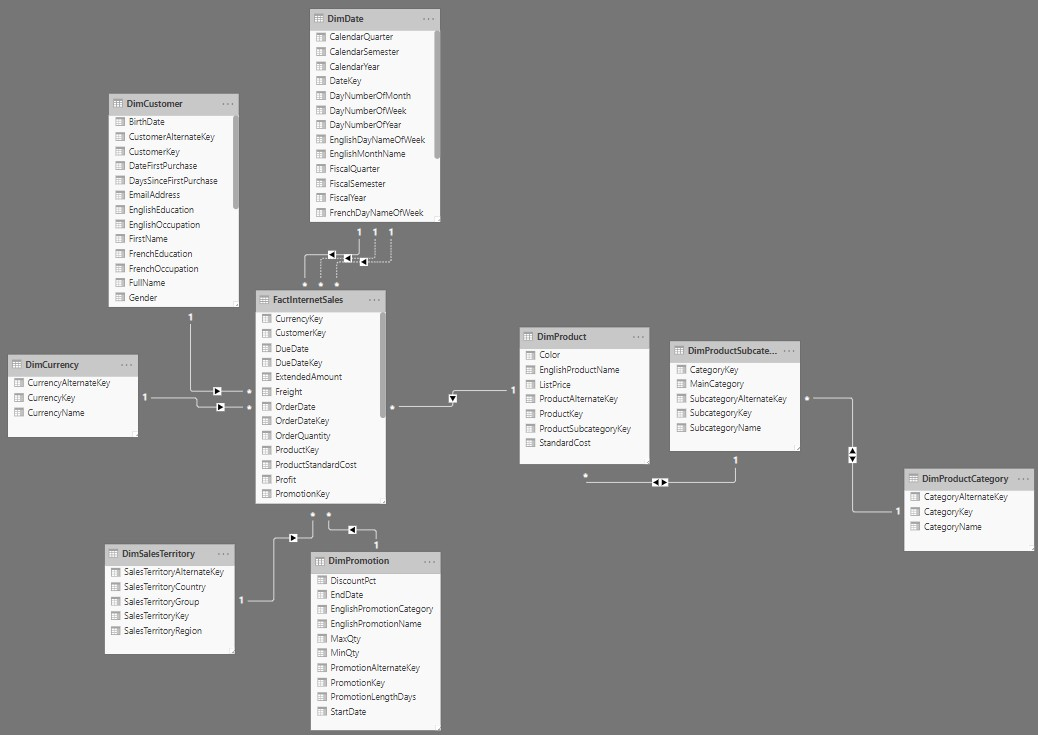
\includegraphics[width=16cm]{./Imagenes/imgpbi1} 
	\end{center}
\end{itemize} 